% \section{Estado del arte}
\section{State of the Art}

% La monitorización de la fauna silvestre mediante imágenes aéreas ha evolucionado significativamente, pasando de métodos de conteo manual propensos a sesgos humanos a sistemas automatizados basados en visión por computador. La revisión de la literatura revela una transición tecnológica desde las Redes Neuronales Convolucionales (CNN) tradicionales hacia arquitecturas especializadas en densidad y, más recientemente, hacia modelos basados en Transformers y mecanismos de atención. A continuación, se describen los enfoques más relevantes y la evolución técnica que fundamenta este proyecto.
Wildlife monitoring through aerial imagery has evolved significantly, transitioning from manual counting methods prone to human biases to automated systems based on computer vision. The literature review reveals a technological transition from traditional Convolutional Neural Networks (CNNs) toward density-specialized architectures and, more recently, toward Transformer-based models and attention mechanisms. Below, we describe the most relevant approaches and the technical evolution that underlies this project.

% \subsection{Detección basada en CNNs y limitaciones en manadas densas}
\subsection{CNN-based Detection and Limitations in Dense Herds}

% Históricamente, la detección de animales en imágenes aéreas se ha abordado mediante detectores de objetos de propósito general basados en anclas (\textit{anchor-based}), como Faster R-CNN, Libra R-CNN y RetinaNet. Estudios previos sobre el mismo conjunto de datos utilizado en esta investigación demostraron que modelos como Libra R-CNN podían alcanzar una precisión media (mAP) del 80\% en condiciones ideales \cite{delplanque-data}.
Historically, animal detection in aerial images has been approached using general-purpose anchor-based object detectors, such as Faster R-CNN, Libra R-CNN, and RetinaNet. Previous studies on the same dataset used in this research demonstrated that models like Libra R-CNN could achieve a mean Average Precision (mAP) of 80\% under ideal conditions \cite{delplanque-data}.

% Sin embargo, como sintetizan diversas revisiones del campo \cite{xu-review}, estas arquitecturas presentan dos limitaciones fundamentales en el contexto de manadas densas:
However, as synthesized by various field reviews \cite{xu-review}, these architectures present two fundamental limitations in the context of dense herds:

% 1. Dependencia del NMS: el algoritmo de Supresión de No Máximos tiende a eliminar detecciones válidas cuando varios animales aparecen muy próximos, lo que provoca subconteo sistemático.
1. NMS Dependency: the Non-Maximum Suppression (NMS) algorithm tends to eliminate valid detections when several animals appear in close proximity, causing systematic undercounting.

% 2. Objetos pequeños y ocluidos: en imágenes aéreas, los animales suelen ocupar pocos píxeles, y las CNN tradicionales tienen dificultades para distinguir individuos contiguos en fondos heterogéneos.
2. Small and occluded objects: in aerial images, animals typically occupy few pixels, and traditional CNNs have difficulty distinguishing contiguous individuals against heterogeneous backgrounds.

% En estudios aplicados a fauna africana, Delplanque et al. observaron caídas críticas de precisión en grupos densos debido exactamente a estos factores \cite{delplanque-data}. Estas limitaciones motivaron el desarrollo de modelos específicamente diseñados para entornos con oclusión extrema.
In studies applied to African wildlife, Delplanque et al. observed critical drops in precision in dense groups due to exactly these factors \cite{delplanque-data}. These limitations motivated the development of models specifically designed for environments with extreme occlusion.

% \subsection{HerdNet y el enfoque basado en puntos}
\subsection{HerdNet and the Point-based Approach}

% Para resolver el dilema entre la localización precisa y el conteo en masas, Delplanque et al. propusieron \textbf{HerdNet}, el cual se establece como el modelo de referencia (\textit{baseline}) para este proyecto \cite{herdnet}. HerdNet abandona el enfoque de cajas delimitadoras en favor de una estimación basada en puntos, inspirada en técnicas de conteo de multitudes (\textit{crowd counting}).
To resolve the dilemma between precise localization and mass counting, Delplanque et al. proposed \textbf{HerdNet}, which is established as the baseline model for this project \cite{herdnet}. HerdNet abandons the bounding box approach in favor of point-based estimation, inspired by crowd counting techniques.

% Esta arquitectura utiliza un mapa de Transformada de Distancia Inversa Focal (FIDT).Este mapa genera picos localizados en el centro de cada animal, permitiendo detectar individuos incluso cuando no hay contornos claros, evitar por completo el uso de NMS, y mantener robustez en presencia de oclusiones y variaciones de escala.
This architecture uses a Focal Inverse Distance Transform (FIDT) map. This map generates localized peaks at the center of each animal, enabling the detection of individuals even when there are no clear contours, completely avoiding the use of NMS, and maintaining robustness in the presence of occlusions and scale variations.

% Aunque HerdNet superó a las arquitecturas basadas en anclas (como Faster R-CNN) y basadas en densidad pura (como DLA-34) con un F1-Score del 73.6\% y un RMSE de 9.8, sobre el conjunto de datos de múltiples especies utilizado en este proyecto, presenta desafíos en la clasificación de especies minoritarias y una dependencia de arquitecturas de CNN convencionales que pueden no capturar eficazmente el contexto global de la imagen.
Although HerdNet outperformed anchor-based architectures (such as Faster R-CNN) and pure density-based architectures (such as DLA-34) with an F1-Score of 73.6\% and an RMSE of 9.8 on the multi-species dataset used in this project, it presents challenges in classifying minority species and a dependence on conventional CNN architectures that may not effectively capture the global context of the image.

% \subsection{La revolución de los Transformers: WildlifeMapper, OpenWildlife y RF-DETR}
\subsection{The Transformer Revolution: WildlifeMapper, OpenWildlife, and RF-DETR}

% La incorporación de arquitecturas tipo \textit{Transformer} ha marcado un punto de inflexión en la detección de objetos en imágenes aéreas. A diferencia de las CNN convencionales, estos modelos introducen mecanismos de atención capaces de capturar relaciones espaciales de largo alcance, lo que resulta crítico para manejar variaciones extremas de escala y fondos heterogéneos.
The incorporation of \textit{Transformer}-type architectures has marked a turning point in object detection in aerial images. Unlike conventional CNNs, these models introduce attention mechanisms capable of capturing long-range spatial relationships, which is critical for handling extreme scale variations and heterogeneous backgrounds.

% \subsubsection*{WildlifeMapper y OpenWildlife}
\subsubsection*{WildlifeMapper and OpenWildlife}
% Kumar et al. presentaron \textbf{WildlifeMapper} \cite{wildlife-mapper}, una arquitectura que integra módulos de refinamiento local para capturar estructuras de alta frecuencia. Este enfoque ha demostrado ser superior en el manejo de imágenes aéreas de muy alta resolución (hasta $8400 \times 5500$ px), permitiendo una localización precisa en paisajes vastos.
Kumar et al. presented \textbf{WildlifeMapper} \cite{wildlife-mapper}, an architecture that integrates local refinement modules to capture high-frequency structures. This approach has proven superior in handling very high-resolution aerial images (up to $8400 \times 5500$ px), enabling precise localization in vast landscapes.

% Por otro lado, Patel et al. propusieron \textbf{OpenWildlife} \cite{open-wildlife}, un detector de vocabulario abierto basado en la arquitectura \textit{Grounding-DINO}. Este modelo combina un \textit{backbone} visual (Swin Transformer) con un codificador de lenguaje (BERT), permitiendo la detección de fauna guiada por descripciones textuales naturales. Si bien ofrece una gran capacidad de generalización hacia especies no vistas durante el entrenamiento, su arquitectura pesada conlleva un costo computacional que limita su escalabilidad en análisis masivos.
On the other hand, Patel et al. proposed \textbf{OpenWildlife} \cite{open-wildlife}, an open-vocabulary detector based on the \textit{Grounding-DINO} architecture. This model combines a visual \textit{backbone} (Swin Transformer) with a language encoder (BERT), enabling wildlife detection guided by natural textual descriptions. While it offers great generalization capacity toward species not seen during training, its heavy architecture entails a computational cost that limits its scalability in massive analyses.

% \subsubsection*{RF-DETR: Eficiencia en Tiempo Real}
\subsubsection*{RF-DETR: Real-Time Efficiency}
% Más recientemente, Robinson et al. introdujeron \textbf{RF-DETR} \cite{rf-detr}, un \textit{Detection Transformer} diseñado específicamente para optimizar el equilibrio entre precisión y latencia. Esta arquitectura se distingue por dos innovaciones clave:
More recently, Robinson et al. introduced \textbf{RF-DETR} \cite{rf-detr}, a \textit{Detection Transformer} designed specifically to optimize the balance between accuracy and latency. This architecture is distinguished by two key innovations:

\begin{itemize}
    % \item \textbf{Búsqueda de Arquitectura Neuronal (NAS) de peso compartido:} Permite ajustar dinámicamente la profundidad del decodificador, el número de \textit{queries} y las ventanas de atención sin necesidad de reentrenar el modelo desde cero.
    \item \textbf{Weight-shared Neural Architecture Search (NAS):} Allows dynamically adjusting the decoder depth, number of \textit{queries}, and attention windows without needing to retrain the model from scratch.
    % \item \textbf{Backbone DINOv2 \cite{dinov2}:} Incorpora representaciones visuales robustas obtenidas mediante un preentrenamiento autosupervisado a escala de internet.
    \item \textbf{DINOv2 Backbone \cite{dinov2}:} Incorporates robust visual representations obtained through internet-scale self-supervised pretraining.
\end{itemize}

% En benchmarks estándar como COCO y el complejo RF100-VL, RF-DETR ha superado a detectores modernos como YOLOv8 y D-FINE, logrando métricas superiores a 60 AP con latencias por debajo de los 40 ms \cite{rf-detr}. Crucialmente para este proyecto, RF-DETR opera como un detector \textit{end-to-end}, eliminando la necesidad de algoritmos de post-procesamiento manuales como la Supresión de No Máximos (NMS). Esta característica lo hace teóricamente superior en escenarios de alta densidad, donde el NMS tradicional tiende a suprimir individuos contiguos.
On standard benchmarks such as COCO and the complex RF100-VL, RF-DETR has surpassed modern detectors like YOLOv8 and D-FINE, achieving metrics above 60 AP with latencies below 40 ms \cite{rf-detr}. Crucially for this project, RF-DETR operates as an \textit{end-to-end} detector, eliminating the need for manual post-processing algorithms such as Non-Maximum Suppression (NMS). This characteristic makes it theoretically superior in high-density scenarios, where traditional NMS tends to suppress contiguous individuals.

% \subsection{Análisis, brechas identificadas y propuesta}
\subsection{Analysis, Identified Gaps, and Proposal}

% La revisión exhaustiva de la literatura permite identificar tres brechas tecnológicas principales que limitan el monitoreo automatizado de fauna en la actualidad:
The exhaustive review of the literature allows us to identify three main technological gaps that currently limit automated wildlife monitoring:

\begin{enumerate}
    % \item \textbf{Precisión limitada en densidad extrema:} Los modelos tradicionales basados en anclas (como la familia YOLO o Faster R-CNN) fallan sistemáticamente en la detección de manadas densas. Esto se debe intrínsecamente al uso de NMS, que al intentar eliminar duplicados, elimina erróneamente detecciones válidas de animales que se superponen o están muy próximos entre sí \cite{xu-review}.
    \item \textbf{Limited precision in extreme density:} Traditional anchor-based models (such as the YOLO family or Faster R-CNN) systematically fail in detecting dense herds. This is intrinsically due to the use of NMS, which, when attempting to eliminate duplicates, erroneously eliminates valid detections of animals that overlap or are in very close proximity to each other \cite{xu-review}.

    % \item \textbf{Dilema entre localización y contexto semántico:} Enfoques como HerdNet \cite{herdnet} resolvieron eficazmente el problema de la oclusión mediante la estimación de densidad basada en puntos. Sin embargo, al depender de CNNs tradicionales, su capacidad para capturar el contexto global de la imagen es limitada, lo que afecta su capacidad de generalización y clasificación fina en entornos complejos.
    \item \textbf{Dilemma between localization and semantic context:} Approaches like HerdNet \cite{herdnet} effectively solved the occlusion problem through point-based density estimation. However, by relying on traditional CNNs, their ability to capture the global context of the image is limited, affecting their generalization capacity and fine-grained classification in complex environments.

    % \item \textbf{Costo computacional de los modelos fundacionales:} Aunque métodos recientes como WildlifeMapper y OpenWildlife ofrecen un desempeño excelente y capacidades de vocabulario abierto, sus requerimientos computacionales son prohibitivos para el despliegue en escenarios de conservación con recursos limitados o para el procesamiento de grandes volúmenes de datos de drones \cite{open-wildlife}.
    \item \textbf{Computational cost of foundation models:} Although recent methods like WildlifeMapper and OpenWildlife offer excellent performance and open-vocabulary capabilities, their computational requirements are prohibitive for deployment in resource-limited conservation scenarios or for processing large volumes of drone data \cite{open-wildlife}.
\end{enumerate}

% \textbf{Síntesis y propuesta de valor:}
\textbf{Synthesis and value proposal:}
% El análisis de estas limitaciones sugiere que existe una oportunidad no explorada en la intersección de estas tecnologías. Se plantea que la implementación de \textbf{RF-DETR} en el contexto de manadas densas podría cerrar estas brechas simultáneamente.
The analysis of these limitations suggests that there is an unexplored opportunity at the intersection of these technologies. It is proposed that the implementation of \textbf{RF-DETR} in the context of dense herds could close these gaps simultaneously.

% La hipótesis central es que la capacidad de los Transformers para modelar relaciones globales y prescindir del NMS permitirá mejorar la recuperación (\textit{recall}) de individuos en manadas densas, superando el conteo de HerdNet. Simultáneamente, se espera que el uso de un \textit{backbone} robusto como DINOv2 mejore la discriminación entre especies (reduciendo la confusión reportada en HerdNet), todo ello manteniendo una eficiencia computacional viable para su aplicación práctica.
The central hypothesis is that the ability of Transformers to model global relationships and dispense with NMS will improve the recovery (\textit{recall}) of individuals in dense herds, surpassing HerdNet's counting. Simultaneously, it is expected that the use of a robust \textit{backbone} like DINOv2 will improve discrimination between species (reducing the confusion reported in HerdNet), all while maintaining computationally viable efficiency for practical application.

\begin{figure*}[t!]
    \centering
    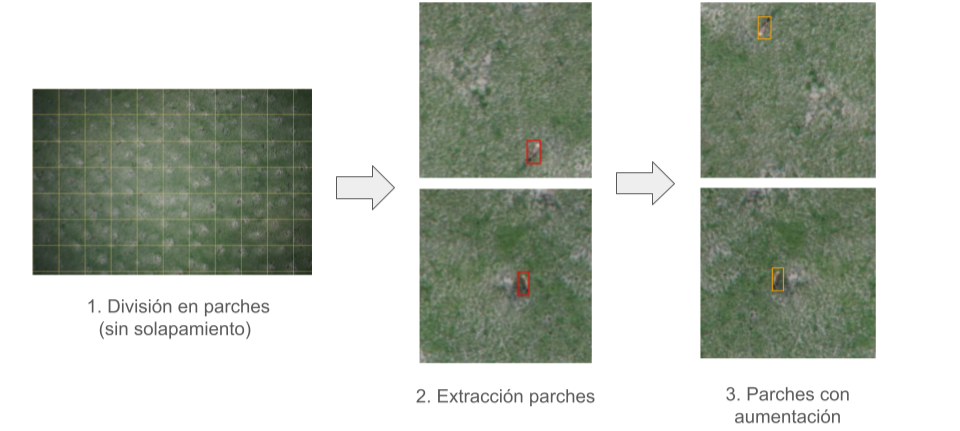
\includegraphics[width=0.8\textwidth]{static/img/aumento.png}
    % \caption{Visualización del preprocesamiento: extracción de recortes (tiling) y ejemplos de aumentación de datos aplicados para el entrenamiento de HerdNet y RF-DETR.}
    \caption{Preprocessing visualization: tile extraction (tiling) and examples of data augmentation applied for HerdNet and RF-DETR training.}
    \label{fig:preprocessing}
\end{figure*}
